%%%%%%%%%%%%%%%%%%%%%%%%%%%%%%%%%%%%%%%%%%%%%%%%%%%%%%%%%%%
%                                                         %
%       This is documentation for the IFJ project.        %
%                                                         %
%%%%%%%%%%%%%%%%%%%%%%%%%%%%%%%%%%%%%%%%%%%%%%%%%%%%%%%%%%%


%------------------------------------------------%
%	    CONFIGURATION + IMPORTED PACKAGES        %
%------------------------------------------------%
\documentclass[12pt,a4paper,titlepage]{article}
\usepackage[english]{babel}
\usepackage[utf8]{inputenc}


\usepackage{graphicx}   % Import pictures

\usepackage{ragged2e}   % fullfill paragraphs

\begin{document}
%-----------------------------------------%
%	            TITLE PAGE                %
%-----------------------------------------%
\begin{titlepage}

\begin{center}
% Headings
\textsc{\LARGE Brno University of technology}\\[0.5cm]
\textsc{\large Faculty of Information Technology}\\[7cm]

% Title - lines
{ \huge \bfseries IFJ project}\\[0.3cm]
{ \Large \bfseries documentation}\\[0.4cm]
{\bfseries xbenes49, xbolsh00, xpolan09}\\[12cm]

% Date
\today
\end{center}

\end{titlepage}
\newpage

%-----------------------------------------%
%	         TABLE OF CONTENTS            %
%-----------------------------------------%

\tableofcontents  % The table of contents
\thispagestyle{empty}
\newpage


%-----------------------------------------%
%	            CHAPTERS                  %
%-----------------------------------------%

\setcounter{page}{1}
\pagenumbering{arabic}

\section{Lexical analysis}

\begin{justify}
We did the scanner in two ways: singlethread and multithread work. Both variants work on the basis of a state machine.
The state machine was created on a basis of regular expression designs for each type of phrasems:
integer, real number (decimal point, positive or negative exponent), string, operator, identifier, keyword, comment.

The multithread scanner implementation used separate thread, read bytes from input, generates tokens and pushes
them to the queue. The parser then reads from the queue and processess the tokens in it. At some moment of multithread
implementing, we have come to the decision, that the singlethread scanner would be better, since we have got one member off.

For the purpose of decomposition, the structure of the lexical analyzer was divided into several subprograms
that implemented individual parts.
\end{justify}

%%%%% getNumber %%%%%
\begin{justify}
Numbers, decimal and exponential numbers are scanned in the function \textit{getNumber()}.
\end{justify}
\begin{center}
  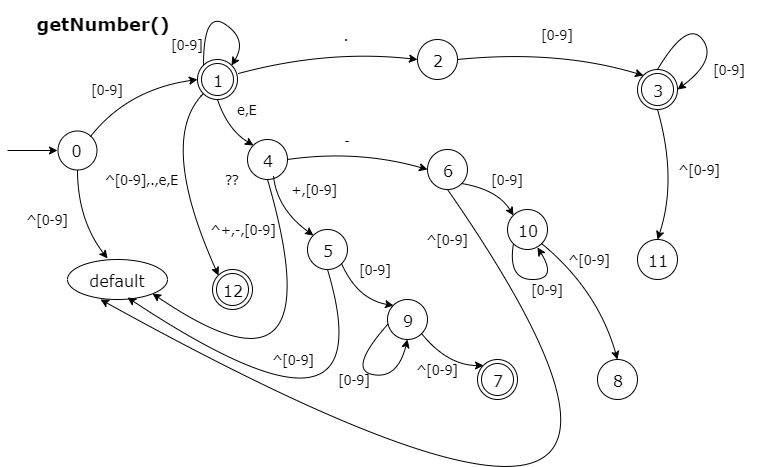
\includegraphics[width=0.7\textwidth]{img/getNumber.png}
\end{center}

%%%%% getString %%%%%
\begin{justify}
Strings are scanned in the function \textit{getString}.
\end{justify}
\begin{center}
  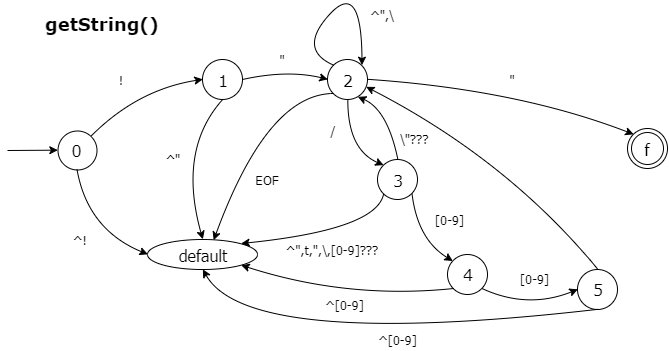
\includegraphics[width=0.7\textwidth]{img/getString.png}
\end{center}

%%%%% getComment %%%%%
\begin{justify}
The comments are scanned in the function \textit{getComment()}. We have simplified the "//" with "\textasciitilde".
\end{justify}
\begin{center}
  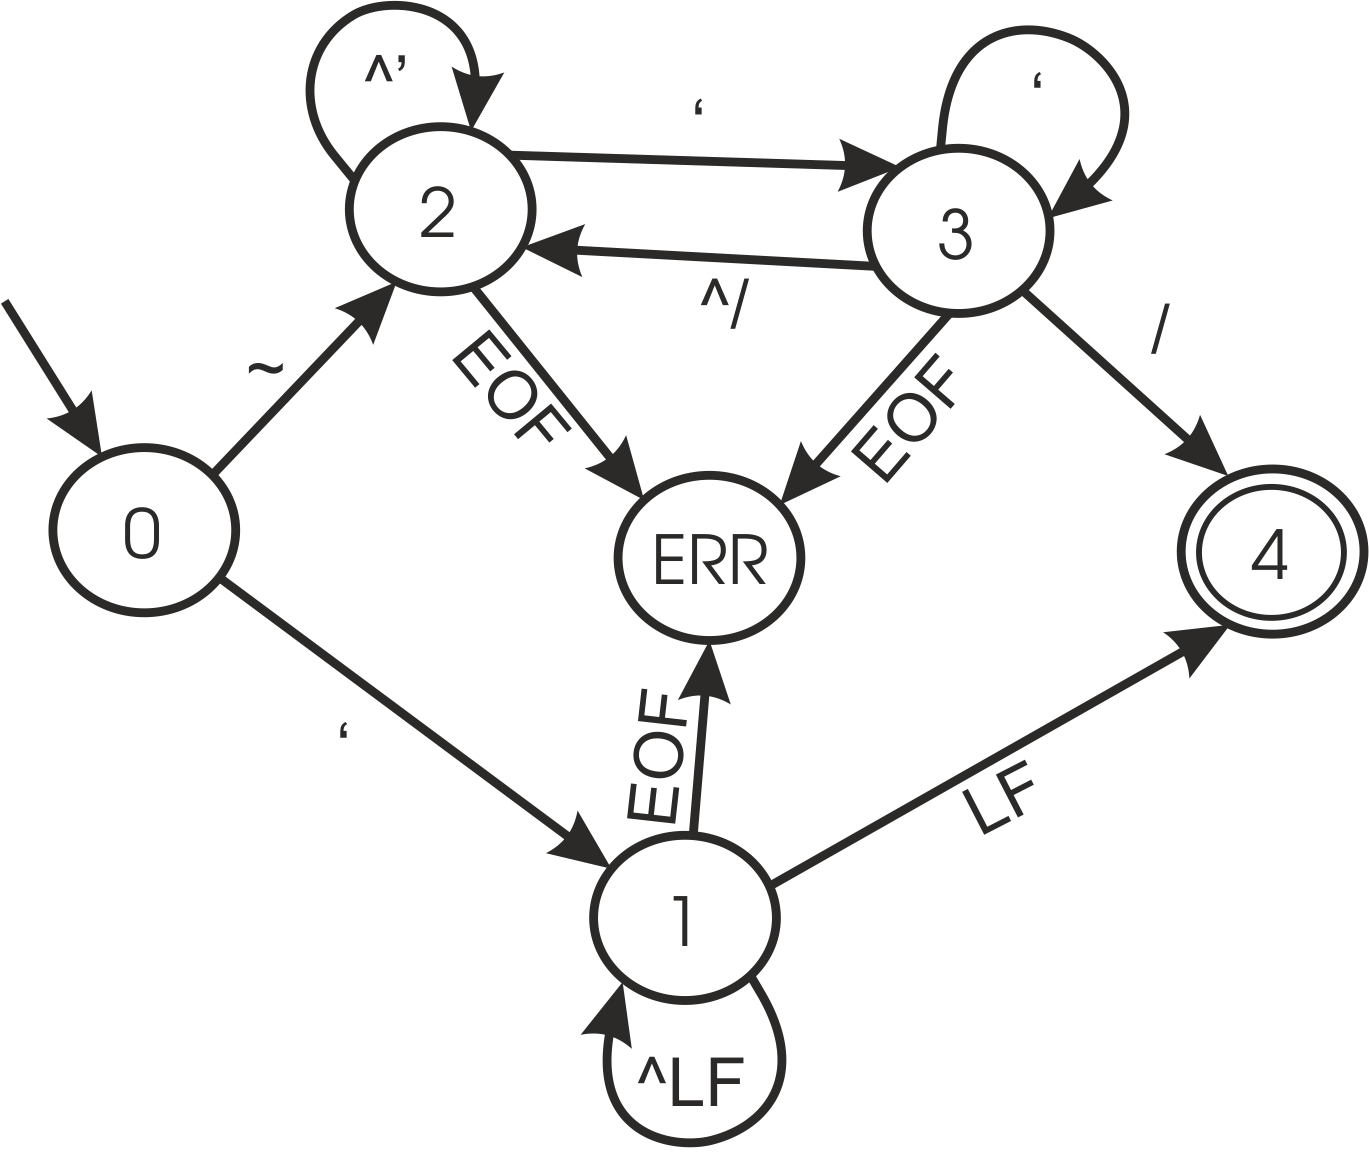
\includegraphics[width=0.7\textwidth]{img/getComment.png}
\end{center}

%%%%% getComment %%%%%
\begin{justify}
Identifiers and keywords are scanned in the function \textit{getIdentifier()}.
\end{justify}
\begin{center}
  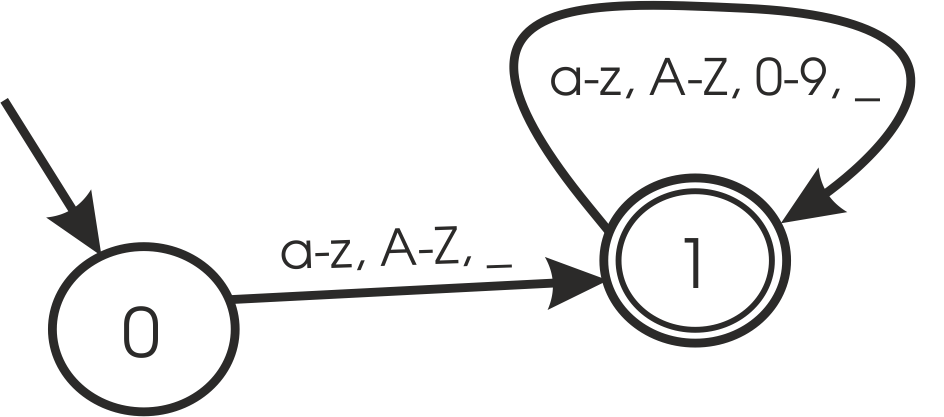
\includegraphics[width=0.7\textwidth]{img/getIdentifier.png}
\end{center}

%%%%% getComment %%%%%
\begin{justify}
Operators are scanned in the function \textit{getOperator()}
\end{justify}
\begin{center}
  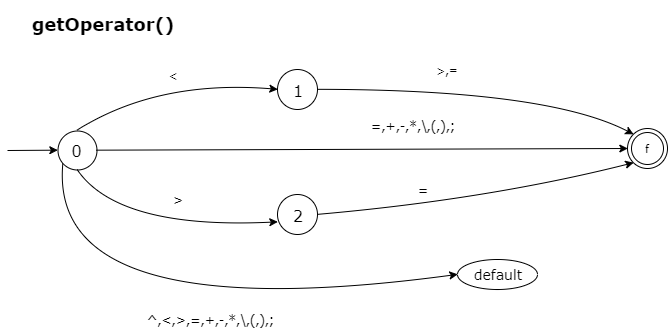
\includegraphics[width=0.7\textwidth]{img/getOperator.png}
\end{center}

\begin{justify}
To simplify the implementation, we use a wrapper modul \textit{io.h} to
be able to return bytes back to the input with the function \textit{returnByte()}.
\end{justify}

\newpage
% ------------------------------------------------------- %

\section{Parser}

% LL table
\begin{center}
  \begin{tabular}{ | l | c  c  l | } \hline
    1  & $<$GlobalBlock$>$              & $\rightarrow$ & $<$FunctionDeclaration$>$ $<$GlobalBlock$>$ \\ \hline
    2  & $<$GlobalBlock$>$              & $\rightarrow$ & $<$FunctionDefinition$>$ $<$GlobalBlock$>$ \\ \hline
    3  & $<$GlobalBlock$>$              & $\rightarrow$ & $<$Scope$>$ $<$GlobalBlock$>$ \\ \hline
    4  & $<$GlobalBlock$>$              & $\rightarrow$ & $\varepsilon$ \\ \hline
    5  & $<$FunctionDeclaration$>$      & $\rightarrow$ & {\it declare} $<$FunctionHeader$>$ \\ \hline
    6  & $<$FunctionDefinition$>$       & $\rightarrow$ & $<$FunctionHeader$>$ $<$Block$>$ $<$EndFunction$>$ \\ \hline
    7  & $<$FunctionHeader$>$           & $\rightarrow$ & {\it function} $<$FSymbol$>$ {\it (} $<$Parameters$>$ {\it )} {\it as} $<$DataType$>$ {\it \$} \\ \hline
    8  & $<$Scope$>$                    & $\rightarrow$ & {\it scope} {\it \$} $<$Block$>$ $<$EndScope$>$ \\ \hline
    9  & $<$FSymbol$>$                  & $\rightarrow$ & {\it id} \\ \hline
    10 & $<$VSymbol$>$                  & $\rightarrow$ & {\it id} \\ \hline
    11 & $<$DataType$>$                 & $\rightarrow$ & {\it string} \\ \hline
    12 & $<$DataType$>$                 & $\rightarrow$ & {\it double} \\ \hline
    13 & $<$DataType$>$                 & $\rightarrow$ & {\it integer} \\ \hline
    14 & $<$EndFunction$>$              & $\rightarrow$ & {\it end} {\it function} {\it \$} \\ \hline
    15 & $<$EndScope$>$                 & $\rightarrow$ & {\it end} {\it scope} {\it \$} \\ \hline
    16 & $<$Parameters$>$               & $\rightarrow$ & $<$VSymbol$>$ {\it as} $<$DataType$>$ $<$MoreParameters$>$ \\ \hline
    17 & $<$MoreParameters$>$           & $\rightarrow$ & {\it ,} $<$Parameters$>$ \\ \hline
    18 & $<$MoreParameters$>$           & $\rightarrow$ & $\varepsilon$ \\ \hline
    19 & $<$Block$>$                    & $\rightarrow$ & $<$VariableDefinition$>$ $<$Block$>$ \\ \hline
    20 & $<$Block$>$                    & $\rightarrow$ & $<$Assignment$>$ $<$Block$>$ \\ \hline
    21 & $<$Block$>$                    & $\rightarrow$ & $<$Input$>$ $<$Block$>$ \\ \hline
    22 & $<$Block$>$                    & $\rightarrow$ & $<$Print$>$ $<$Block$>$ \\ \hline
    23 & $<$Block$>$                    & $\rightarrow$ & $<$Condition$>$ $<$Block$>$ \\ \hline
    24 & $<$Block$>$                    & $\rightarrow$ & $<$Cycle$>$ $<$Block$>$ \\ \hline
    25 & $<$Block$>$                    & $\rightarrow$ & $<$Return$>$ $<$Block$>$ \\ \hline

  \end{tabular}
\end{center}


\end{document}

\begin{table}
\begin{tabular}{*8l}
\X\alpha        &\X\theta       &\X o           &\X\tau         \\
\X\beta         &\X\vartheta    &\X\pi          &\X\upsilon     \\
\X\gamma        &\X\gamma       &\X\varpi       &\X\phi         \\
\X\delta        &\X\kappa       &\X\rho         &\X\varphi      \\
\X\epsilon      &\X\lambda      &\X\varrho      &\X\chi         \\
\X\varepsilon   &\X\mu          &\X\sigma       &\X\psi         \\
\X\zeta         &\X\nu          &\X\varsigma    &\X\omega       \\
\X\eta          &\X\xi                                          \\
                                                                \\
\X\Gamma        &\X\Lambda      &\X\Sigma       &\X\Psi         \\
\X\Delta        &\X\Xi          &\X\Upsilon     &\X\Omega       \\
\X\Theta        &\X\Pi          &\X\Phi
\end{tabular}
\caption{Greek Letters}\label{greek}
\end{table}
